\documentclass[10pt,twocolumn,letterpaper]{article}

\usepackage{cvpr}
\usepackage{times}
\usepackage{epsfig}
\usepackage{graphicx}
\usepackage{amsmath}
\usepackage{amssymb}

% Include other packages here, before hyperref.

% If you comment hyperref and then uncomment it, you should delete
% egpaper.aux before re-running latex.  (Or just hit 'q' on the first latex
% run, let it finish, and you should be clear).
\usepackage[breaklinks=true,bookmarks=false]{hyperref}

\newcommand{\todo}[1]{\textcolor{red}{[Todo: #1]}}

\cvprfinalcopy % *** Uncomment this line for the final submission

\def\cvprPaperID{****} % *** Enter the CVPR Paper ID here
\def\httilde{\mbox{\tt\raisebox{-.5ex}{\symbol{126}}}}

% Pages are numbered in submission mode, and unnumbered in camera-ready
%\ifcvprfinal\pagestyle{empty}\fi
%\setcounter{page}{4321}
\begin{document}

%%%%%%%%% TITLE
\title{Pooling Pyramid Network for Object Detection}

\author{
Pengchong Jin
\hspace*{32pt}
Vivek Rathod
\hspace*{32pt}
Xiangxin Zhu
\\
Google AI Perception\\
{\tt\small \{pengchong, rathodv, xiangxin\}@google.com}
}


\maketitle
%\thispagestyle{empty}

%%%%%%%%% ABSTRACT
\begin{abstract}
  We'd like share a simple tweak of the Single Shot Multibox Detector
  (SSD) family of detectors,
  which is effective in reducing the model size while
  maintaining the same quality. We share the box predictors
  across all the scales, and replace the convolution between
  scales with max pooling. This has two advantages over
  SSD: (1) avoids score miscalibration across scales; (2)
  the shared predictor sees the training data over all
  scales. Since we reduce the number of predictor to one, and
  trim all the convolutions between them, the model size is
  significantly small. We empirically show that these changes
  does not hurt the model quality compared to SSD.

\end{abstract}

%%%%%%%%% BODY TEXT
\section{Introduction}
SSD detectors~\cite{liu2016ssd,lin2017focal} have
been popular as they run fast, are simple to implement
and easily portable to different types of hardware.


Most of the SSD detectors have several feature maps
representing different scales, each of which uses its own
predictor to produce the boxes and class scores.
In practice, especially when the data distribution is skewed
over scales, this design is problematic. Imagine a
dataset with tons of large objects and very few small ones.
The predictors from small scale feature maps will be
wasted as they rarely see any positives. This data imbalance
could also result in score miscalibration across scale even
for the same class. Another issue with this design is that
each predictor only sees the objects at its own scale. This
partition will divide the already small dataset
into even smaller sets. If we believe the object
appearance is scale invariant, it will be a more efficient
if all the predictors see all of the data.

We propose simple changes to SSD: use the same predictor
for all scales. In order for the predictor to work in the
same feature space, we replace the convolutions between
feature maps with max pooling.

%\section{Related Work}

%Multibox~\cite{erhan2014multibox}



%YOLO~\cite{redmon2016yolo}

%YOLO-v2~\cite{redmon2017yolov2}

%FPN~\cite{lin2017fpn}

%Survey~\cite{huang2017gmi}


\section{Pooling Pyramid Network (PPN)}
The proposed model, \textit{Pooling Pyramid Network (PPN)},
is a single-stage convolutional object detector, very
similar to SSD with simple changes.  The prediction head is
designed to be light-weight, fast to run, while maintaining
comparable detection accuracy with SSD.
The network architecture is illustrated in
Figure~\ref{fig:ppn}.  There are two major changes to
original SSD~\cite{liu2016ssd}: (1) the box predictor is
shared across feature maps with different scales; (2) the
convolutions between feature maps are replaced with the max
pooling operations.  In the following sections, we will
discuss the rationale behind these changes and discuss their effects.

\begin{figure*}[t]
\begin{center}
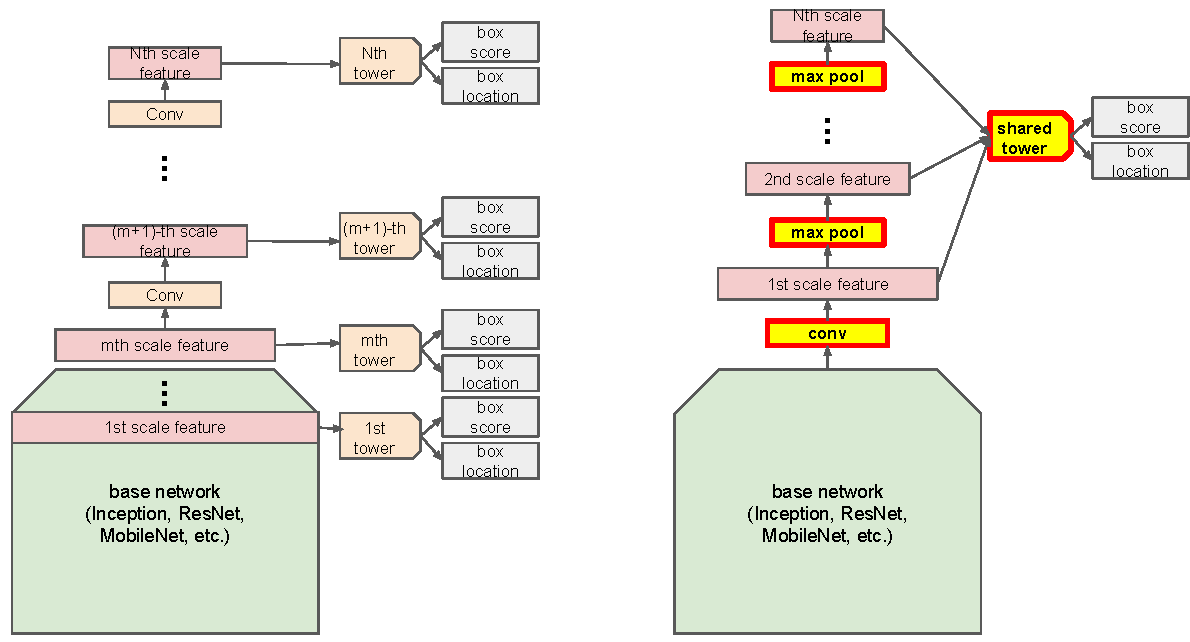
\includegraphics[width=1.0\linewidth]{figure/ppn_vs_ssd.pdf}
\end{center}
\caption{
The architecture comparison between the Pooling Pyramid Network (PPN)
and SSD. Left: SSD, Right: PPN.
Note that the changes in PPN are highlighted:
(1) using max pool to build the feature pyramid,
(2) using shared convolutional predictor for box classification and regression.
}
\label{fig:ppn}
\end{figure*}

\subsection{Shared Box Predictor}
SSD uses independent box predictors for feature maps at different scales.
One problem is miscalibration of the prediction scores across different scales.

Since each box predictor is trained independently using only
a portion of the groundtruth boxes that it is assigned to,
different box predictors could see very different amount of
positive and negative examples during the training.  This
implicit data imbalance causes the problem that scores
from different predictors fall in vastly different ranges,
which makes them incomparable and difficult to use in the
subsequent score-based postprocessing steps such as non maximum
suppression.  We design PPN with a shared box predictor
across feature maps of different scales.  As a result, the
box predictor sees all of the training data during even when
there is an imbalance in groundtruth box scales. This reduces
the effect of miscalibration and unstable prediction scores.

One could argue that having separate box predictor for each
scale increases the total capacity, and allows each
predictor to focus at its specific scale. However, we think
hat this may not be necessary as objects are mostly scale
invariant. In practice, Faster-RCNN~\cite{ren2015frcnn}
works well with a single shared predictor.


\subsection{Max Pooling Pyramid}

Our goal is to build a multi-scale feature pyramid
structure, from which we can make the predictions using the
shared box predictor.  We achieve this by shrinking down a
base feature map from the backbone network several times
using a series of max pooling operations.  This is different
from SSD where feature maps are built by extracting layers
from backbone network and shrinking them using additional
convolutions, and FPN where feature maps are built by a
top-down pathway with skip connections.  We choose max
pooling mainly for two reasons.  First, using the pooling
operations ensures feature maps with different scales live
in the same embedding space, which makes training the shared
box predictor more effective.  In addition, since max
pooling does not require any additions and multiplicatons,
it is very fast to compute during the inference, therefore,
making it suitable for many latency sensitive applications.

One may use the seemingly more intuitive avearge pooling
to build the feature pyramid.
It should be noted, however, that
nonlinear operations after pooling need to be inserted,
because otherwise it is a linear operations so that
scores from the lower level feature maps would be higher than
those from the pooled ones.
We haven't experimented with the average pooling yet.

% (1) avoids score miscalibration across scales, which
%  could be a problem if the object size distribution is
%  skewed and each scale makes independent predictions; (2)
%  the shared predictor sees the training data over all
%  scale.

\begin{table*}[t]
\begin{center}
\begin{tabular}{l|c|c|c|c}
Model & mAP & inference FLOPs & number of parameters & GPU inference time\\
\hline
\hline
MobileNet SSD & 20.0 & 2.48B & 6.83M & 27ms \\
\hline
MobileNet PPN & 19.7 & 2.35B & 2.18M & 26ms \\
\end{tabular}
\end{center}
\caption{COCO detection: MobileNet SSD vs MobileNet PPN}
\label{comparison}
\end{table*}



\subsection{Overall Architecture}


The final network architecture of our Pooling Pyramid
Network (PPN) detector is illustrated in
Figure~\ref{fig:ppn}.  Followed by the backbone network, an
optional $1\times 1$ convolution is used to transform the features
from the backbone network to a space with desired
dimensions.  We then apply a series of stride-2 max pooling
operations to shrink the feature map down to $1\times 1$.  A shared
box predictor is applied to feature maps of different scales
in order to produce classification scores and location
offsets of box predictions.  We add one additional shared
convolution in the box predictor after pooling operations to
prepare the feature to be used for predictions.


\section{Experiments}

We run the experiments on COCO~\cite{lin2014coco} detection dataset
and compare the performance of PPN with SSD.
We use MobileNet v1~\cite{howard2017mobilenet} as the backbone network
and set the input resolution to be $300\times 300$.
Both models use the standard implementation of MobileNet-v1 SSD in
Google Object Detection API~\cite{huang2017gmi}.
For PPN,
we extract the layer \textit{Conv2d\_11\_pointwise} as the base feature map,
from which we build 6 pooled feature maps that are of sizes
$19\times 19$,
$10\times 10$,
$5\times 5$,
$3\times 3$,
$2\times 2$, and
$1\times 1$.
A shared $1\times 1$ depth 512 convolution is applied before the box classifier and location regressor.
We use the similar anchor design as SSD,
the smooth $l_{1}$ loss for box regression,
and the focal loss with $\alpha=0.25$ and $\gamma=2$ for box classification.
Our implementation is based on Google Object Detection API
and it is publicly available under Tensorflow's Github repository.

Both SSD and PPN models are initialized using the MobileNet-v1 checkpoint
that is pre-trained on ImageNet, and
both of them are trained and tested on the splits described in
~\cite{huang2017gmi}.
We leverage Google Cloud TPU for fast training.
We perform the model benchmark using an Nvidia GeForce GTX TITAN X card.
Table \ref{comparison} shows the comparison between SSD and PPN.
PPN achieves the similar mAP (19.7 vs 20.0),
comparable FLOPs and inference time,
but 3x smaller in model size.

%\todo{Can we have the model size, FLOPs of both the whole
%models and the prediction head in the table?
%Xiangxin@, I am not sure if this is worth to put here.
%For model size, it seems obvious that people would know the reduction comes from the head (sharing).
%For FLOPs, I am not sure it's benefitical to break it down.
%Their numbers are very close (sharing won't change the FLOPs becaue it doesn't reduce the computation).
%WDYT
%}


{\small
\bibliographystyle{ieee}
\bibliography{refs}
}

\end{document}
